\documentclass[letterpaper, 10pt, conference]{ieeeconf}

\IEEEoverridecommandlockouts    % If we want to use the thanks command

\usepackage{color}
\usepackage{graphicx}
\usepackage{amsmath}
\usepackage{amssymb}
\usepackage{url}
\usepackage{subfig}

% EPS2PDF stuff?

\newcommand{\xxx}[1]{\textcolor{red}{#1}}

\title{\LARGE \bf
    3D Environment Reconstruction Using RGB-D Visual Odometry
}

\author{Pedro D'Aquino, Rob Goeddel, Lauren Hinkle, and John Peterson}


\begin{document}

\maketitle
%\thispagestyle{empty} % XXX These were in the IROS example, but I didn't read
                      % far enough along to see if they disappear later
%\pagestyle{empty}

\begin{abstract}
The reconstruction of environments in 3D can be challenging with just range
data. RGB-D sensors like the Microsoft Kinect provide visual details that
allow odometry to be used even in environments with ambiguous depth data.
This paper demonstrates a simplified implementation of Henry et al.'s work
on RGB-D Mapping.~\cite{Henry2010rgbd}
Our system can construct reasonably accurate models of
small to medium sized indoor environments in real time at resolutions of up
to 2\,cm and in near-real time at 1\,cm. By using SURF features from the image
data in conjunction with the Kinect's depth data, we are able to compute
accurate alignments of point clouds over time. Our system does not attempt to
implement the loop-closing portion of Henry et al.'s work.
\end{abstract}

\section{Introduction and Motivation}
This paper will present a system capable of building detailed colored point
clouds using a consumer grade RGB-D sensor, the Microsoft Kinect. The
convenient availability of such sensors makes them an appealing budget option
for a small robot operating in an indoor environment where the limited range
of the Kinect is less of a concern. Furthermore, the colored point data
generated by RGB-D sensors can provide more robust alignments than even high
quality pure-range sensors such as LIDAR in environments with range-detectable
features.

LIDAR and other range based sensors may be used to generate extremely detailed
and accurate 3D point clouds that may be merged over time to reconstruct a 3D
model of an environment. Generally, these alignments are straightforward to
detect and such systems are fairly robust. However, there are some weaknesses.
A classic example is the so-called ``hallway problem.'' A common concern for
SLAM systems is that all stretches of a long hallway look the same. The lack
of distinguishing features mean that, while we may correctly align the walls
to run parallel to previously observed walls, it is difficult if not
impossible to constrain an observation to one particular location. Depending
on the reliability of a robot's odometry, this may cause compression or
expansion of the hallway in question. Features from associated image data can
make an otherwise indistinguishable segment of wall easy to align with
previous scans, as seen in Fig.~\ref{fig:cse-wall}.

The output of an RGB-D sensor can also be used for general 3D modeling
applications. Artists may spend days creating detailed models of objects from
the real world. Given an RGB-D sensor and a system capable of merging many
observations, an untrained user can wave the sensor around the object needing
to be modeled and automatically generate a 3D model complete with texture.
This preservation of visual data even aids in the end product of the mapping
task. Imagine a 3D map of a building created from range data. While the map
might be an accurate layout of the building, the lack of visual cues may still
leave the user feeling lost and confused while navigating through a virtual
reconstruction of this environment. Associated color data could
have features such as door numbers and maps of the building available to aid
in navigation.

% Figure spanning columns. Top of second page, probably
\begin{figure*}[t]
\centering
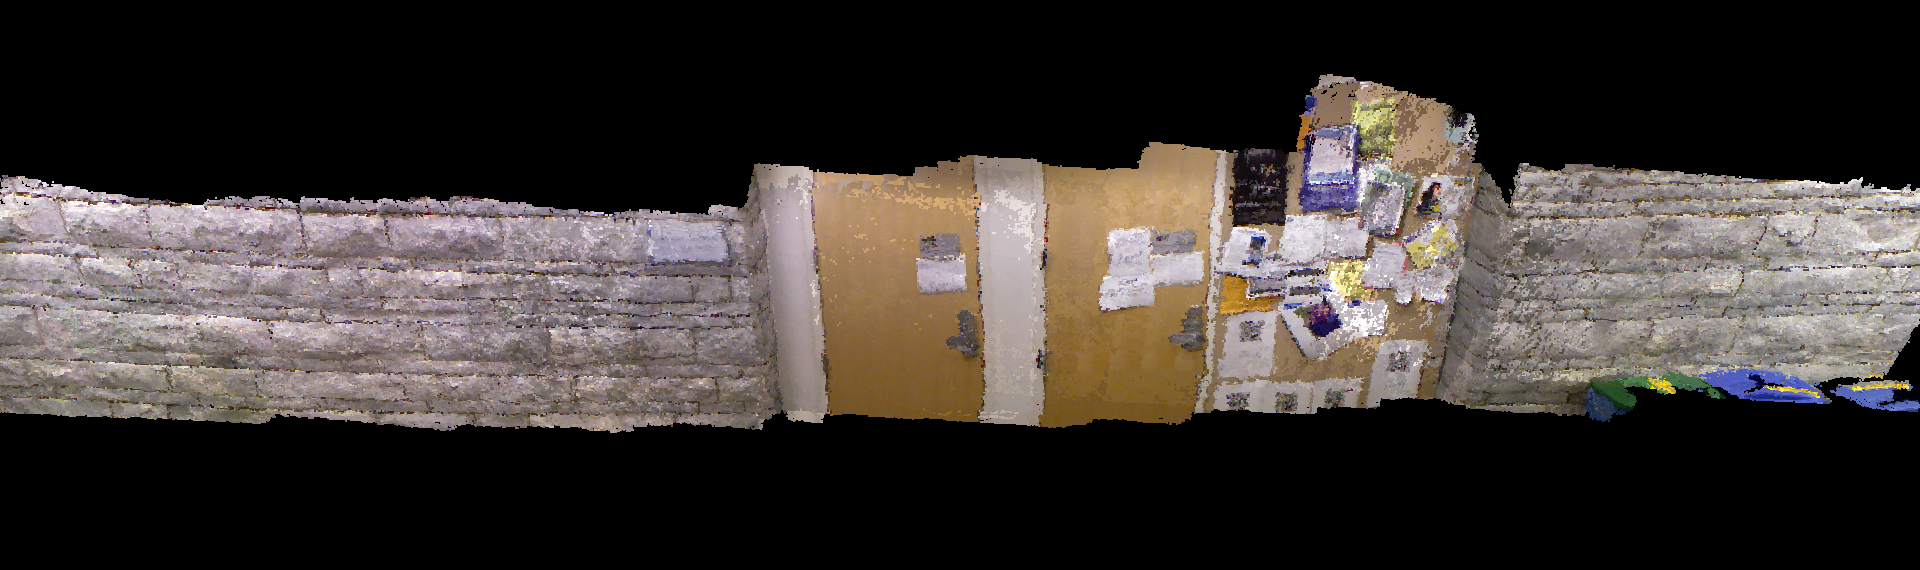
\includegraphics[width=.9\textwidth]{figures/CSE_Wall.png}
\caption{By using image features such as the corners of rocks in a wall,
combined color and depth data can be accurately placed into a global map even
in flat hallway situations. As seen above, even when depth features such as
the doorways and recycling bins go out of view, our system continues to build
an accurate model of the wall to the left of the doors.}
\label{fig:cse-wall}
\end{figure*}

\section{Background}
Our work is a simplified reimplementation of the work of Peter Henry et
al~\cite{Henry2010rgbd}. Their work demonstrated a system capable of RGB-D
mapping using a conjunction of 3D SIFT alignment, plane-fitting ICP, and the
SLAM system TORO. By using visual features projected into 3D space to gain an
initial alignment between frames and by using ICP to converge the rest of the
way, Henry et al. were able to make a ``near-real time'' system capable of
producing very detailed 3D reconstructions. By maintaining periodic keyframes
for different locations, they are able to make large-scale loop closures by
recognizing those same features later, resulting in a very robust system.

To show their results, Henry et al. created what they call \emph{surfels}.
Surfels allow them to deal with the massive amounts of data provided by their
RGB-D sensor without losing significant detail about the scene. As videos of
their results demonstrate, the system is capable of preserving details such as
the pattern on carpet or slightly blurry versions of people's faces in
pictures.

Albert Huang and his group at MIT, working in conjunction with Henry et al. at
the University of Washington, were able to take this system a step further,
creating a real-time mapping system that allowed a quadrotor to autonomously
fly through cluttered 3D environments using a Kinect~\cite{Huang2011isrr}.
Huang et al.'s work adds data from IMUs and switches to FAST features to
support real time voxel mapping at a coarse resolution sufficient for
trajectory planning.

\section{Methodology}
\xxx{METHODOLOGY GOES HERE}
Our implementation of RGB-D mapping passes entirely on the SLAM portion,
focusing instead on feature-based odometry. Lacking time to implement a
full RGB-D SLAM system capable of rendering real-time navigable scenes at the
level of detail demonstrated by Henry et al., we focused on making our system
real-time. This can be used to justify many of deviations from the original
implementation.

\subsection{Kinect Data Acquisition and Calibration}
We use the open source OpenKinect library (often referred to as libfreenect)
to acquire data from the Kinect~\cite{OpenKinect}. Though our project is
written primarily in Java, our interface to the Kinect is written in C and we
use JNI bindings to tie the C and java together. We are easily able to acquire
a full 30 frames per second with this code.

We calibrated our Kinect using Nicolas Burrus's RGBDemo
toolkit~\cite{BurrusCalibration}. The software includes a tool for calibrating
a Kinect simply by taking a large number of pictures of a calibration target
with both the IR and RGB cameras. This tool not only returns the intrinsics
and undistortion parameters for both cameras, but also the stereo calibration
parameters relating the two cameras to each other. Using these parameters
along with a depth model provided by Dr. St\'{e}phane Magnenat on the
OpenKinect website, we are able to construct a colored point cloud with only
minimal blurring of color between objects.

\subsection{Frame Matching Using Image Features}
The first approximation of the movement of the Kinect comes from matching 3D image
features between the current and the last frame. In this section, we describe the details
of our implementation.

\subsubsection{Feature Extraction and Description}
We compute SURF features and descriptors
to extract and describe features in the image~\cite{Bay06surf}. Our approach differs
from Henry et al., who use a parallel implementation of SIFT descriptors~\cite{SIFTGPU}.
As the majority of the development laptops we used had integrated graphics cards, using
a GPU implementation was not feasible. We found that SURF was an adequate tradeoff
between robustness and performance. Our implementation uses OpenCV~\cite{opencv_library}
for feature detection and descriptor extraction, with a JNI wrapper to allow for
communication with the rest of the system.

\subsubsection{Feature Matching}
We match a SURF feature to its nearest Euclidian neighbor in the other frame. The matching
uses a kd-tree for efficiency. We experimented with reducing the number of outliers by
constraining the matches in two ways. In the ``distant second'' approach, let $A_i$ be the
best match for feature $B_j$, with distance $d_{ij}$, and $A_k$ be the second best match,
with distance $d_{kj}$. Then we only consider $A_i$ to match $B_j$ if $d_{ij} \le \alpha d_{jk}$.
We also experimented with enforcing ``marriage'' between matches: $A_i$ matches $B_j$ only if
$B_j$ also matches $A_i$.

Both constraints reduced the number of wrong matches, but also eliminated some inliers.
Additionaly, there was significant overhead from applying the ``marriage'' constraint.
In the end, we found that applying RANSAC as explained in the next section was enough
to robustly filter outliers.

\subsubsection{Computing the Rigid Body Transformation}
\label{ransac}
Once we extract these features from the RGB images, we project them into 3D space
using the depth data from the Kinect. Given these 3D SURF features, we may
compute good alignment using RANSAC and Horn's algorithm. \xxx{Lauren, talk
    more about point alignment}

\subsection{ICP}
Once we've used RANSAC to gain an initial alignment, we use ICP to jiggle the
new frame into place. \xxx{John, talk about ICP here!}

\subsection{Rendering the Scene}
We do not attempt to implement the surfels demonstrated by Henry et al.
Surfels, while excellent at preserving detail, are a huge engineering
undertaking in and of themselves, and even so, it is extremely costly to
update their values during data collection. Surfels alone would destroy our
chances of rendering in real time. Instead, we choose to store data as voxel
of a fixed resolution. Voxel updates are practically free, and individual
voxels do not change in memory requirements over time. Our voxels store a
running total of the ARGB values observed in that bin and are treated as
being colored as an average of these observations.

Henry et al. wrote a custom tool to allow them to navigate surfel environments
in real time~\cite{Henry2010rgbd}. Again, this was a large engineering effort
and was not our main priority. Instead, we attempted to render all of our
voxels at once, regardless of on screen visibility. The performance for this
rendering scheme proved to be unacceptable, so our voxels are instead rendered
as individual points rendered at the center of their respective bins. As a
result, scenes are best viewed from some distance so as to mask the gaps
between the points. To facilitate 3D navigation through the scene, we employ a
logitech gamepad supporting XYZ translate rotation around each of these axes
relative to the current camera position.

\section{Evaluation}
\xxx{EVALUATION AND PRETTY FIGURES GO HERE}
\subsection{Ground Truth Evaluation}

\subsection{Performance}

\begin{figure}
\centering
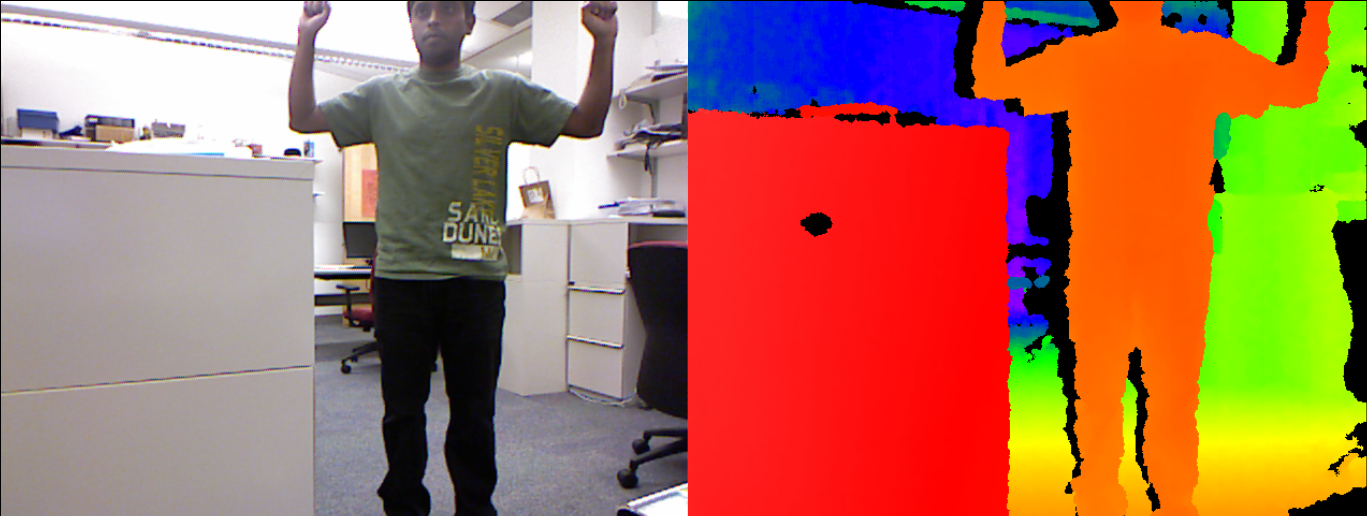
\includegraphics[width=0.48\textwidth]{figures/KinectDemo.png}
\caption{RGB and depth data from a Kinect. For easier consumption, the depth
data has been mapped through the colors of the rainbow where red corresponds
to objects roughly 1\,m away and purple corresponds to objects roughly 8~\,m
away. Though the maximum range is at least 8\,m, the depth data
becomes increasingly noisy, so we only use data within 3.8\,m of the Kinect,
the range at which the data seems to begin to deteriorate.}
\label{fig:kinect-demo}
\end{figure}

\subsection{Public Demonstration}
To show how our system works, we employ two separate demonstrations. The first
is a simple Kinect testing demo that we used to verify that we were receiving
good color and depth data (seen in Fig.~\ref{fig:kinect-demo}. This demo helps
us explain the type of data that a Kinect gives us and how we can use that to
construct 3D point clouds in the first place. Our second demonstration
consists of running our system live at a slightly lowered resolution so that
point data is clearly added to our model of the world as we move around. By
allowing people to fly through our virtual world as we are actively building
it, they can easily compare the virtual scene to the real one before them. We
can also build detailed 3D models of people on the fly, if the are able to
hold still for a long enough period of time. %Reference to Ed picture

\section{Conclusion}
\xxx{CONCLUSION GOES HERE}

\section*{Acknowledgements}
Special thanks to Pradeep Ranganathan for providing some extra depth
information in Fig.~\ref{fig:kinect-demo}.

% XXX References
\bibliographystyle{IEEEtranS}
\bibliography{sources}

\end{document}
